% !TeX spellcheck = it_IT
\documentclass{llncs}
%%%%%%%%%%%%%%%%%%%%%%%%%%%%%%%%%%%%%%%%%%%%%%%%%%%%%%%%%%%
%% package sillabazione italiana e uso lettere accentate
\usepackage[latin1]{inputenc}
\usepackage[english]{babel}
\usepackage[T1]{fontenc}
%%%%%%%%%%%%%%%%%%%%%%%%%%%%%%%%%%%%%%%%%%%%%%%%%%%%%%%%%%%%%

\usepackage{url}
\usepackage{xspace}
\usepackage{amsmath}
\usepackage{pdfpages}


\makeatletter
%%%%%%%%%%%%%%%%%%%%%%%%%%%%%% User specified LaTeX commands.
\usepackage{manifest}
\usepackage{textcomp}
\makeatother

\usepackage{tikz}
\usetikzlibrary{arrows,automata}

\newcommand{\java}{\textsf{Java}}
\newcommand{\contact}{\emph{Contact}}
\newcommand{\corecl}{\texttt{corecl}}
\newcommand{\medcl}{\texttt{medcl}}
\newcommand{\msgcl}{\texttt{msgcl}}
\newcommand{\android}{\texttt{Android}}
\newcommand{\dsl}{\texttt{DSL}}
\newcommand{\jazz}{\texttt{Jazz}}
\newcommand{\rtc}{\texttt{RTC}}
\newcommand{\ide}{\texttt{Contact-ide}}
\newcommand{\xtext}{\texttt{XText}}
\newcommand{\xpand}{\texttt{Xpand}}
\newcommand{\xtend}{\texttt{Xtend}}
\newcommand{\pojo}{\texttt{POJO}}
\newcommand{\junit}{\texttt{JUnit}}

\newcommand{\action}[1]{\texttt{#1}\xspace}
\newcommand{\code}[1]{{\small{\texttt{#1}}}\xspace}
\newcommand{\codescript}[1]{{\scriptsize{\texttt{#1}}}\xspace}

% Cross-referencing
\newcommand{\labelsec}[1]{\label{sec:#1}}
\newcommand{\xs}[1]{\sectionname~\ref{sec:#1}}
\newcommand{\xsp}[1]{\sectionname~\ref{sec:#1} \onpagename~\pageref{sec:#1}}
\newcommand{\labelssec}[1]{\label{ssec:#1}}
\newcommand{\xss}[1]{\subsectionname~\ref{ssec:#1}}
\newcommand{\xssp}[1]{\subsectionname~\ref{ssec:#1} \onpagename~\pageref{ssec:#1}}
\newcommand{\labelsssec}[1]{\label{sssec:#1}}
\newcommand{\xsss}[1]{\subsectionname~\ref{sssec:#1}}
\newcommand{\xsssp}[1]{\subsectionname~\ref{sssec:#1} \onpagename~\pageref{sssec:#1}}
\newcommand{\labelfig}[1]{\label{fig:#1}}
\newcommand{\xf}[1]{\figurename~\ref{fig:#1}}
\newcommand{\xfp}[1]{\figurename~\ref{fig:#1} \onpagename~\pageref{fig:#1}}
\newcommand{\labeltab}[1]{\label{tab:#1}}
\newcommand{\xt}[1]{\tablename~\ref{tab:#1}}
\newcommand{\xtp}[1]{\tablename~\ref{tab:#1} \onpagename~\pageref{tab:#1}}
% Category Names
\newcommand{\sectionname}{Section}
\newcommand{\subsectionname}{Subsection}
\newcommand{\sectionsname}{Sections}
\newcommand{\subsectionsname}{Subsections}
\newcommand{\secname}{\sectionname}
\newcommand{\ssecname}{\subsectionname}
\newcommand{\secsname}{\sectionsname}
\newcommand{\ssecsname}{\subsectionsname}
\newcommand{\onpagename}{on page}

\newcommand{\student}{Zanotti Andrea}
\newcommand{\studentEmail}{andrea.zanotti9}
\newcommand{\xfaculty}{II Faculty of Engineering}
\newcommand{\xunibo}{Alma Mater Studiorum -- University of Bologna}
\newcommand{\xaddrBO}{viale Risorgimento 2}
\newcommand{\xaddrCE}{via Venezia 52}
\newcommand{\xcityBO}{40136 Bologna, Italy}
\newcommand{\xcityCE}{47023 Cesena, Italy}

%
% Comments
%
%%% \newcommand{\todo}[1]{\bf{TODO:}\emph{#1}}


\begin{document}

\title{Button Led System\\
 process report}

%%% \author{\xauthA \and \xauthB}
\author{\student}

\institute{%
%%%  \xunibo\\\xaddrCE, \xcityCE\\\email{\{nameA.studentA, nameB.studentB\}@studio.unibo.it}
  \xunibo\\\xaddrBO, \xcityBO\\\email\ {\studentEmail}@studio.unibo.it
}

\maketitle

%% \begin{abstract}
%% \footnotesize
%%This a Latex template to be used for the reports of Software Engineering.
%%\keywords{Software engineering, managed software development, reports, ....}
%%\end{abstract}

%%% \sloppy

%===========================================================================
\section{Introduction}
\labelsec{intro}
%===========================================================================

%===========================================================================
\section{Vision}
Non esiste codice senza progetto, non esiste progetto senza analisi del problema e non esiste problema senza requisiti.\\
Non c'� codice senza test.\\
Button e Led sono metafore per input e output.\\
Mantenere disaccopiati logica realizzativa del progetto e testing.\\
Individuare diverse tipologie di test da applicare in diversi momenti della realizzazione:
\begin{itemize}
\item Unit testing (singolo componente, white box)
\item Integration Testing (di interazione, white box)
\item Functional Testing (sull'intero sistema, black box)
\item Stress Load Testing (performance, black box)
\item User Acceptance Testing (feedback utente, black box)
\end{itemize}
Utilizzare approccio top-down in fase di progettazione e bottom-up in fase di implementazione (zooming).\\
Zooming: sviluppo del progetto senza curarsi delle tecnologie che verranno utilizzate per implementarlo.\\
Il Button Led System deve essere una applicazione compatibile con IoT.\\
Rendere l'applicazione Button Led System funzionante a prescindere dalla posizione, dalla tecnologia d'implementazione e dalla tecnologia utilizzata per la comunicazione (ICT).\\
Realizzare il progetto seguendo le linee guida del framework SCRUM.\\
Sempre nell'ambito delle linee guida SCRUM, all'interno dello sprint backlog, devono essere individuate funzionalit\`a utili all'intera software house, che verranno (nello sprint successivo) fattorizzate e rese disponibili come libreria.
Realizzazione di una entit\`a esterna che esegue la configurazione dell'intero Button Led System in modo autonomo e configurabile, in modo da non delegare ai componenti il compito della configurazione.\\
Abbattere i costi per un prodotto di qualit\`a: raggiunti i requisiti minimi di funzionalit\`a continuare a investire risorse nel progetto per aumentarne la qualit\`a e abbatterne i costi.
\labelsec{Vision}
%===========================================================================

%===========================================================================
\section{Goals}

Implementare ogni componente del ButtonLedSystem (button, led e controller) su piattaforma:
\begin{itemize}
	\item Android
	\item Raspberry
	\item Arduino
	\item Java SE
\end{itemize}
\labelsec{Goals}
%===========================================================================

%===========================================================================
\section{Requirements}
\labelsec{Requirements}
Design and build a ButtonLed software system in which a Led is turned on and off each time a Button is pressed (by an human user). The system should run on a single support, e.g. a conventional PC, a Raspberry Pi or Arduino.
%===========================================================================

 
%===========================================================================
\section{Requirement analysis}
\labelsec{ReqAnalysis}
%===========================================================================
\subsection{Use cases}
\labelssec{UseCases}

\subsection{Scenarios}
\labelssec{Scenarios}

\subsection{(Domain)model}
\labelssec{(Domain)model}
LED:
Struttura: entit� atomica, passiva.\\
Interazione: espone le operazioni void turnOn, void turnOff e boolean getState. Queste operazioni sono anche metodi nell'accezione OOP.\\
Comportamento: alla creazione un LED � spento. L'esecuzione dell'operazione turnOn accende il Led, l'esecuzione dell'operazione turnOff lo spegne. L'operazione getState ritorna lo stato del Led (false \textrightarrow spento, true \textrightarrow acceso).\\
Viene esplicitato dal seguente automa a stati finiti:
\begin{center}
	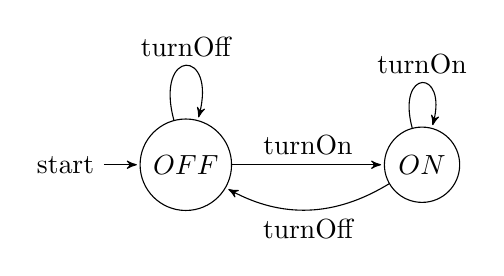
\begin{tikzpicture}[>=stealth',shorten >=1pt,auto,node distance=3cm]
	\node[initial,state] (OFF)      {$OFF$};
	\node[state]         (ON) [right of=OFF]  {$ON$};


	\path[->] (OFF)  edge [loop above] node {turnOff} (OFF)
					 edge              node {turnOn} (ON)
			  (ON)   edge [bend left]  node {turnOff} (OFF)
					 edge [loop above] node {turnOn} (ON);
	\end{tikzpicture}
\end{center}
BUTTON:\\
Struttura: entit� atomica, attiva.\\
Interazione: una sola operazione per conoscere lo stato, boolean getState.\\
Comportamento: alla creazione un button � released.\\
Viene esplicitato dal seguente automa a stati finiti:\\
\begin{center}
	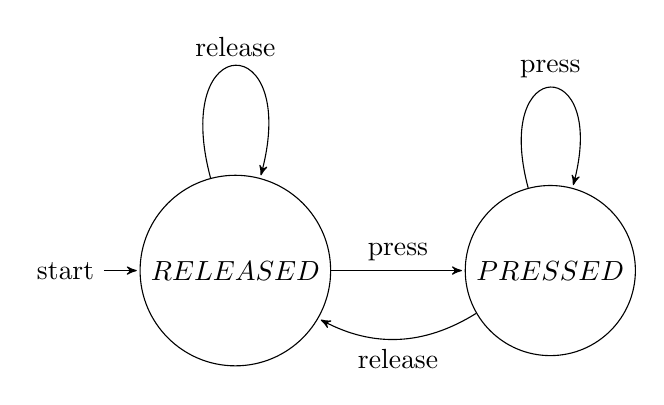
\begin{tikzpicture}[>=stealth',shorten >=1pt,auto,node distance=4cm]
		\node[initial,state] (RELEASED)      {$RELEASED$};
		\node[state]         (PRESSED) [right of=RELEASED]  {$PRESSED$};
		\path[->] (RELEASED)  edge [loop above] node {release} (RELEASED)
							  edge              node {press} (PRESSED)
				  (PRESSED)   edge [bend left]  node {release} (RELEASED)
							  edge [loop above] node {press} (PRESSED);
	\end{tikzpicture}
\end{center}
Button e Led non sono correlati \textrightarrow il button non ha alcuna conoscenza del led e viceversa, per realizzare il sistema � necessaria un'entit� coordinatrice.\\
\subsection{Test plan}
\labelsec{Test plan}
LED:\\
Il test plan (di tipo unit) deve verificare che inizialmente getState ritorni il valore false.
Dopo aver eseguito l'operazione turnOn, getState deve restituire il valore true.\\
BUTTON:\\
\'{E} necessaria una nuova entit� (DebuggableButton) per poter modificare lo stato del button, tale entit� esporra le operazioni, void press, void release.
%===========================================================================
\section{Problem analysis}
\labelsec{ProblemAnalysis}
Per risolvere il problema di scalabilit\`a e mantenere le entit\`a disaccoppiate faremo utilizzo del pattern \texttt{Observer}: il Button espone un'interfaccia tramite la quale le entit\`a possono registrarsi.\\
Dividiamo i componenti dell'architettura in Attivi e Passivi.\\
I componenti Passivi generalmente generano eventi, i componenti Attivi possono ricevere comandi. Per la realizzazione di tale funzionalit\`a verr\`a utilizzato il pattern \texttt{Command}.\\
%\`E inoltre necessario accordarsi su un linguaggio di interazione, il quale necessita di uno standard di comunicazione. Lo standard di comunicazione sar\`a indispensabile per Integration Test.
%===========================================================================
\subsection{Logic architecture}
L'architettura logica \`e esplicitata in figura.
\begin{center}
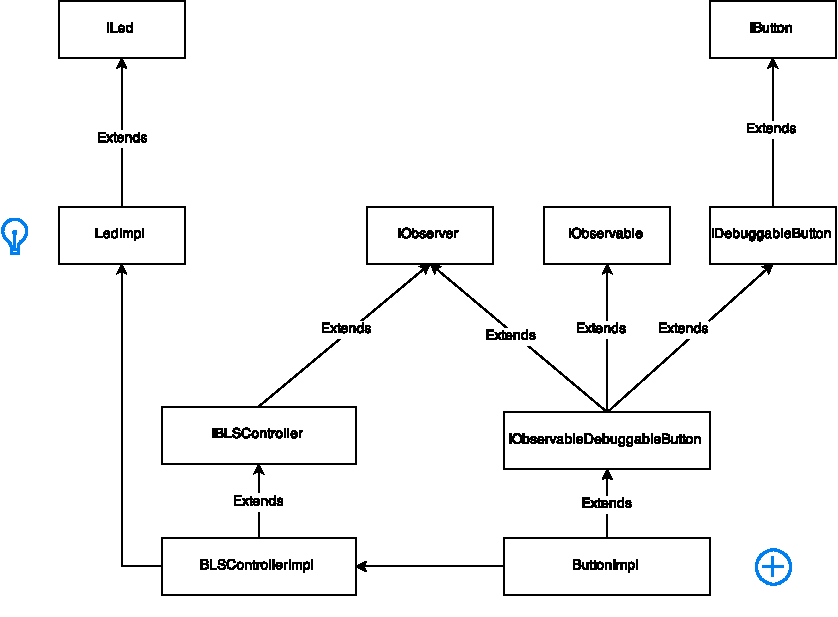
\includegraphics{img/graphs/Analisi_BLS.pdf}
\end{center}
\begin{center}
\end{center}

\subsection{Abstraction gap}

\subsection{Risk analysis}
Nell'interfaccia del Button, oltre al metodo accessor \texttt{isPressed} deve essere presente anche il metodo \texttt{addObserver}, ci\`o \`e risultato necessario dai colloqui con il committente (durante l'analisi dei requisiti).
%===========================================================================
\section{Work plan}
\labelsec{wplan}
%===========================================================================

%===========================================================================
\section{Project}
\labelsec{Project}
L'architettura progettuale \`e esplicitata in figura.
\begin{center}
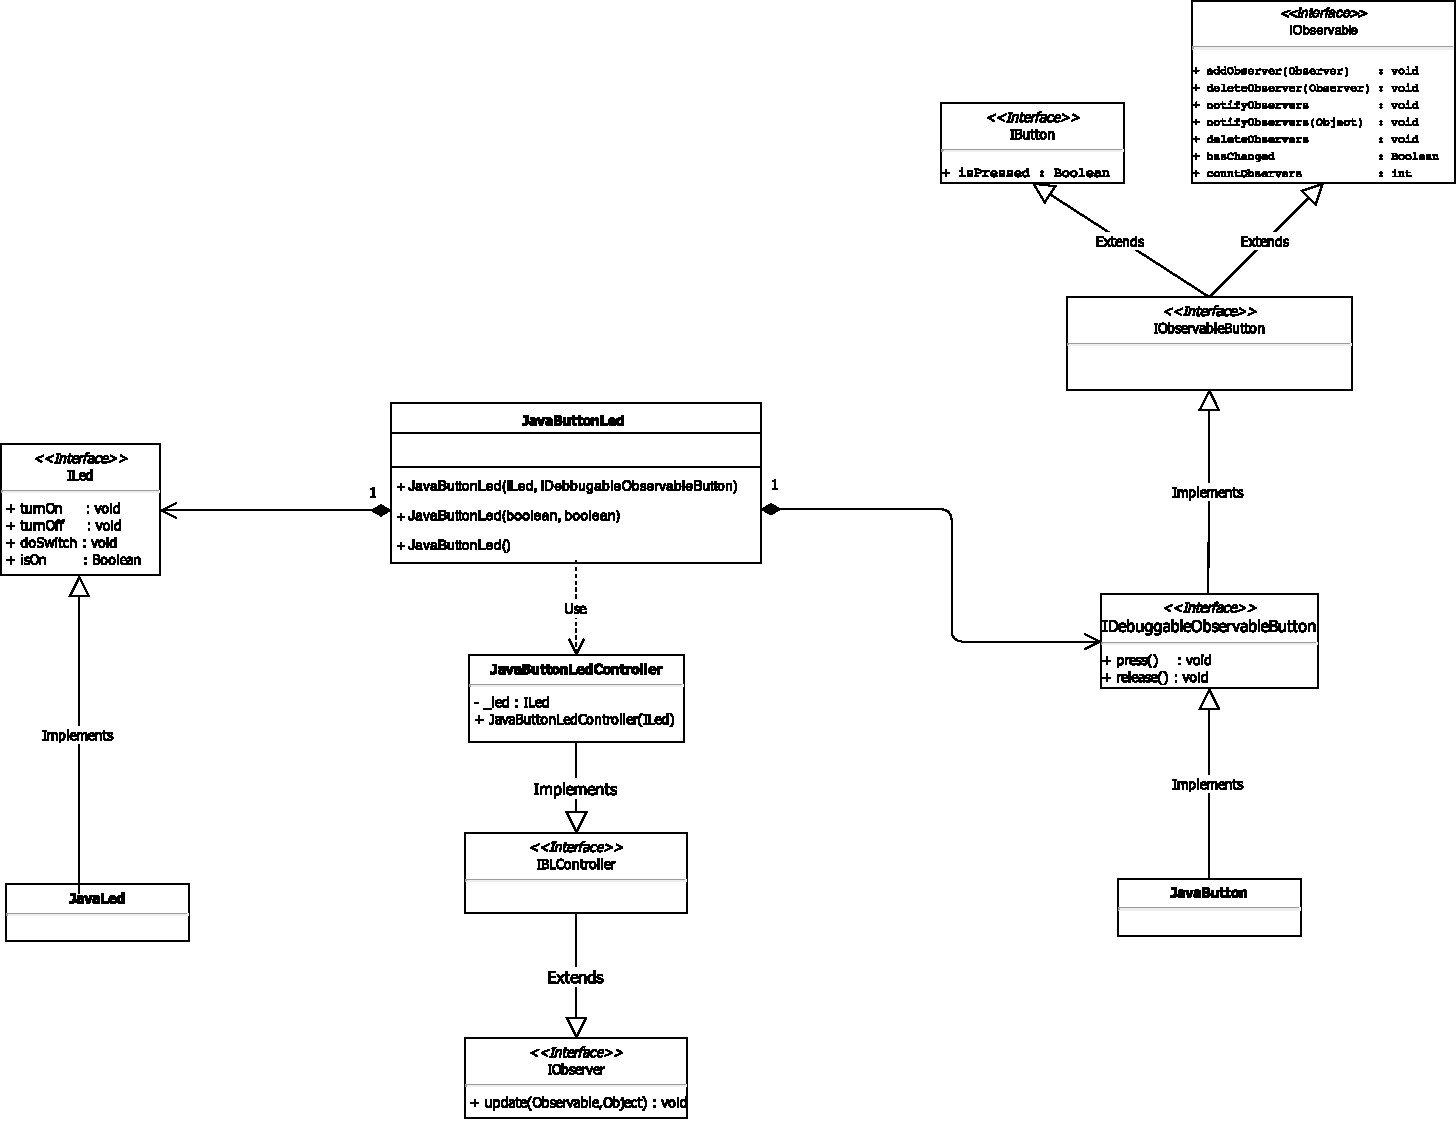
\includegraphics[scale=0.6]{img/graphs/Progettazione_BLS.pdf}
\end{center}
%===========================================================================

\subsection{Structure}
\subsection{Interaction}
\begin{center}
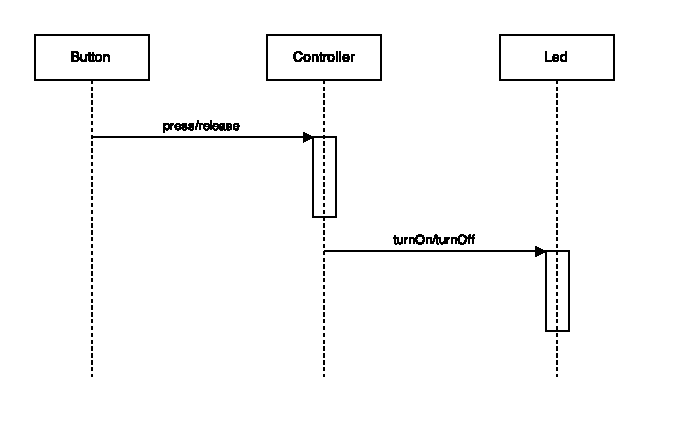
\includegraphics{img/graphs/Interaction.pdf}
\end{center}
\subsection{Behavior}

%===========================================================================
\section{Implementation}
\labelsec{Implementation}
%===========================================================================

%===========================================================================
\section{Testing}
\labelsec{testing}
%===========================================================================

%===========================================================================
\section{Deployment}
\labelsec{Deployment}
%===========================================================================

%===========================================================================
\section{Maintenance}
\labelsec{Maintenance}
%===========================================================================

%===========================================================================
\section{Information about the author}
\labelsec{Author}
%===========================================================================
\newpage
\vskip.5cm
%%% \begin{figure}
\begin{tabular}{ | c |  }
	\hline
	Photo of the Author\\
   	
\includegraphics[width=5cm]{img/zano.jpg}\\
	\hline
\end{tabular}
 
\appendix


\bibliographystyle{abbrv}
\bibliography{biblio}

\end{document}












